\documentclass[../Kamil_Kowalewski_Main.tex]{subfiles}

\begin{document} {

    Ze względu na dynamiczny wzrost, rozwój zagadnień i~tematyki opisanej w~rozdziale
    \ref{chapter1:wstep}, naukowcy nie pozostają w~tyle a~wręcz wiodą prym w~rozwijaniu
    systemów rekomendacji. Jest to dokonywane poprzez opracowywanie nowych metod
    i~przedstawianie śmiałych wizji. Wiele z~tych metod przedstawia nowatorskie pomysły
    oraz wykazuje się wyższą skutecznością niż rozwiązania dostępne w~literaturze.
    Bardzo często jest to poparte badaniami w~publikowanej literaturze. Wydawnictwa
    powszechnie zaliczane do grupy tych najbardziej prestiżowych przeprowadzają
    wnikliwe recenzje przed publikacją co w~większości przypadków gwarantuje wysoką
    jakość przedstawianych treści. Nie mniej ze względu na mnogość dostępnych
    publikacji konieczna staje się weryfikacja ich zawartości celem wyboru takich prac,
    które przedstawiają zagadnienia najbardziej zbliżone do rozważanego problemu.

    \section{Systemy rekomendacji}
    \label{chapter2:przeglad_literatury:systemy_rekomendacji} {
        Celem \textit{Systemów rekomendacyjnych} \cite{website:recommendation_systems}
        (ang. Recommendation Systems) jest automatyzacja doradztwa podczas podejmowania
        złożonych, wieloetapowych decyzji. Podstawą działania tych systemów są
        wcześniej dokonane wybory przez konkretnego użytkownika lub grupę użytkowników,
        do której można zaklasyfikować osobę lub podmiot, na rzecz którego wykonywana
        jest rekomendacja. Systemy te są rozwijane i~wykorzystywane w~wielu liniach
        produktowych takich przedsiębiorstw jak np. Google\cite{website:google} czy też
        Microsoft\cite{website:microsoft}, celem zwiększenia zadowolenia użytkownika
        oraz zysków danej firmy. Nie jest to jedyna możliwość ich wykorzystania, gdyż
        pojęcie \textit{Systemy rekomendacji} jest stosunkowo szerokie. Z~najlepszej
        wiedzy autora niniejszej pracy magisterskiej wynika, że system, który dokonuje
        analizy przekazanych obiektów, a~następnie zwraca użytkownikowi wskazania, czy
        też rekomendacje, co do wyboru jednego lub wielu z~przekazanych obiektów, można
        zaliczyć do tej grupy systemów.
    }

    \section{Określanie wiarygodności ofert oraz rekomendacja tych odpowiednich}
    \label{chapter2:przeglad_literatury:wiarygodnosc_ofert} {
        Proces określania wiarygodności ofert należy do grupy procesów wieloetapowych,
        aby go przeprowadzić, warto pamiętać o~podstawowych definicjach przedstawionych
        w~sekcji \ref{chapter1:wstep:definicje}. Na wiarygodność oferty ma wpływ wiele
        czynników takich jak stosunek proponowanej ceny do ceny rynkowej produktu,
        stosunek pozytywnych i~negatywnych ocen oraz recenzji produktu. Nie mniej
        istotna jest opinia na temat sprzedawcy, która jest ugruntowana na podstawie
        informacji zwrotnych od klientów, którzy dokonywali transakcji u~danego
        sprzedawcy.

        Na podstawie ww. informacji oraz innych czynników jak obecność zdjęć produktu,
        czy też dokładny i~szczegółowy opis, użytkownik wybranego systemu
        informatycznego nakierowanego na e-commerce, może stwierdzić, czy chce zamówić
        danych produkt, czy też nie. Nie jest tajemnicą, że proces ręcznej weryfikacji
        należy do dosyć żmudnych i~czasochłonnych, co nie jest mile widziane
        w~kontekście handlu elektronicznego.

        Warto wspomnieć, że proces ten można zautomatyzować, jak większość procesów
        rekomendacji, na podstawie tożsamych informacji, jakie posiada potencjalna
        osoba dokonująca zakupu. Z~tego powodu obecnie w~literaturze istnieje pewna
        liczba rozwiązań proponowanych przez naukowców, aby zniwelować ten
        nieprzyjazny, dla przeciętnego człowieka, proces, który ma na celu podjęcie
        decyzji czy warto poważnie zainteresować się daną ofertą czy też lepiej jest
        kontynuować poszukiwania.
    }

    \section{System określania wiarygodności oparty na analizie sementycznej treści recenzji}
    \label{chapter2:przeglad_literatury:artykul_1} {
        Artykuł zatytułowany ''Trustworthiness evaluation system in E-Commerce
        context''\cite{article:trustworthiness_evaluation_2016} pochyla się nad tematem
        tworzenia systemów podejmowania decyzji (ang. decision support system) oraz
        systemów reputacji zaufania (ang. Trust Reputation systems), często też
        oznaczane poprzez akronim \textit{TRS}. Jego autorzy w~początkowych fragmentach
        artykułu przedstawiają rozwój, zalety, wygodę zakupów poprzez zróżnicowane
        portale ogłoszeniowe. Na podstawie badań wskazują, że użytkownicy tych portali
        nadal wolą opierać się opiniach i~doświadczeniach innych użytkowników, którzy
        zakupili towar z~określonej oferty lub byli klientami danego sprzedawcy.
        Autorzy wskazują bardzo ciekawą kwestię, która nie jest poruszana bardzo często,
        a~mianowicie to, że wiele parametrów takich jak bezpieczeństwo, jakość obsługi
        może być określana w~bezpośredni sposób za pomocą metryk. W~przypadku oceny
        wiarygodności ofert nie ma możliwości wykonania takiej oceny w~sposób
        bezpośredni, aby otrzymać jeden konkretny wynik na podstawie wybranych parametrów.

        Zwrócona jest uwaga na fakt, że znakomita większość gigantów w~sektorze
        e-commerce zapewnia możliwości przesyłania opinii czy też recenzji, lecz nie
        jest w~żaden sposób określana ich wiarygodność. Problem ten może występować
        z~intencjonalnych lub nieintencjonalnych zachowań klientów, którzy wystawiają
        informację zwrotną niezgodną ze stanem rzeczywistym. Może być to kwestia
        pomyłki lub też celowego działania celem nieuczciwej walki z~konkurencją bądź
        w~celach zarobkowych na rzeczy właśnie innych sprzedawców stosujących zakazane
        praktyki w~handlu. Rzeczą, o~której warto wspomnieć, jest fakt, iż autorzy
        artykułu nie wzięli pod uwagę ważnej metodologii, jaką przyjęły wspominane już
        wielokrotnie portale ogłoszeniowe, a~mianowicie, że opinię lub recenzje może
        wystawić użytkownik, który nie dokonał transakcji. Co więcej, w~przeciwieństwie do
        opinii wystawianych w~ramach np. Google Maps, jedna transakcja daje możliwość
        podzielenia się jedną opinią, a~nie wieloma. Zabezpiecza to jeszcze bardziej
        przed osobami, które dla celów zarobkowych wystawiają oceny.

        Rozwiązanie zaproponowane przez autorów opiera się na analizie semantycznej
        zawartości tekstowej recenzji przekazanych przez użytkowników celem oceny
        produktu lub oferowanej usługi. Wspominają oni, że obecnie w~literaturze było
        wiele prób tworzenia podobnych rozwiązań, lecz z~wykorzystaniem podstawowych
        wartości numerycznych takich jak liczba transakcji klienta, zgodność
        w~przedstawianych opinii, czy też data publikacji danej opinii lub recenzji.

        Szczegółowe kroki proponowanej metody polegają na przeprowadzanie wspomnianej
        już analizy semantycznej, celem określania wydźwięku danej opinii np. czy jest
        pozytywna lub negatywna oraz w~jakim stopniu. Uzyskane w~ten sposób wyniki
        porównywane są z~oceną wystawioną przez użytkownika. Dla przykładu może być to
        5~gwiazdek. W~przypadku znacznej rozbieżności, gdzie jej próg jest definiowany
        jako parametr, opinia taka jest oznaczana jako niewiarygodna. W~kontekście
        wykorzystania tego w~elektronicznym systemie sprzedażowym, wyglądałoby to w~ten
        sposób, że użytkownik przesyła swoją informację zwrotną, dokonywana jest
        analiza zgodnie z~przedstawionym algorytmem i~tylko w~przypadku pozytywnego jej
        wyniku jest ona dodawana do portalu. Skutkuje to jej upublicznieniem oraz
        przeliczeniem dotychczasowych statystyk na temat tego produktu.

        W~bardzo dokładny i~przystępny został opisany sposób implementacji metody.
        Jedna z~najważniejszych procesów, jakim jest analiza semantyczna, została
        określano w~krokach takich jak wstępne przygotowanie tekstu poprzez tokenizację
        oraz inne popularne metody wstępnego przygotowania danych tekstowych. Kolejnym
        krokiem jest skorzystanie z~\textit{SentiWordNet} dostępnego w~bibliotece
        \textit{NLTK}, opisanej w~sekcji
        \ref{chapter4:srodowisko_eksperymentalne:impl_programu:bib:nltk}, dostępnej dla
        języka Python, przedstawionego w~sekcji
        \ref{chapter4:srodowisko_eksperymentalne:impl_programu:jezyk}.

        W artykule został przedstawiony tylko przykładowy zbiór kroków, który
        ma na celu wystawienie opinii czy też recenzji razem z rysunkami obrazującymi
        ten proces. Niestety nie zostały przedstawione żadne badanie, z czego wynika, że
        nie został również przedstawiony żaden zbiór danych.

        Co ważne przedstawioną pomysł oraz metodę można wykorzystać dwojako, pierwszym
        sposobem jest stworzenie zewnętrznego systemu, które określałby wiarygodność
        recenzji, a~na podstawie tych właściwych wyliczał statystyki, dzięki czemu
        możliwe byłoby utworzenie dwóch grup ze zbioru produktów, tych nadających się
        do zakupu oraz nienadających się do zakupu. Drugim sposobem wykorzystania jest
        implementacja tego mechanizmu przez właścicieli pewnego portalu ogłoszeniowego.
        We wspomnianym drugim przypadku autorzy przedstawiają użytkownikom, wcześniej
        przygotowaną pulę recenzji, aby ocenili oni ich poprawność oraz zgodność poprzez
        wybranie przycisku ``Lubię To`` lub ``Nie Lubię Tego``. Na tej podstawie byłoby
        określane intencje osoby przesyłającej opinie, co więcej system łączyłby to
        z~wcześniejszym wynikiem o~wiarygodności użytkownika na podstawie jego opinii.
    }

    \section{Metoda określania wiarygodności ofert na podstawie opinii od wiarygodnych użytkowników}
    \label{chapter2:przeglad_literatury:artykul_2} {
        Artykuł zatytułowany ''A new reputation algorithm for evaluating
        trustworthiness in e-commerce
        context''\cite{article:evaluating_trustworthiness_2013} porusza tematykę
        określania wiarygodności ofert poprzez tworzenie systemów reputacji zaufania
        \textit{TRS}. Zostały w~nim przedstawione, w~bardzo ciekawy sposób, definicje
        związane z~domeną, jaką jest zaufania, wspomniane systemy \textit{TRS} oraz czym
        charakteryzują się \textit{TRS}, stworzone w~solidnym i~przemyślany sposób.

        Następnie zostały przedstawione aktualne osiągnięcia z~tej tematyki, dostępnej
        w~literaturze naukowej. Autorzy artykuły wymieniają wiele prac, które skupiają
        się na propozycjach architektur systemów \textit{TRS}, opartych na rozmaitych
        algorytmach obliczających ocenę reputacji w~oparciu o~sam produkt. Inne prace
        mocno ukierunkowują się na analizę semantyczną informacji zwrotnych, czy też
        recenzji od klientów, którzy zakupili ten oferowany produkt przez konkretnego
        sprzedawcę. Wspomniane jest, że pomimo starań, inne pozycje literaturowe nie
        rozważają wielu problemów, takich jak wiarygodność osób piszących komentarze,
        systematycznej aktualizacji ich wiarygodności, poprzez przechowywania wartości
        np. liczbowej, która mówiłaby o~tym czy w recenzję lub opinię danego użytkownika
        można uwierzyć.

        Niezwykle poruszającą kwestią jest przechodniość zaufania oraz jej związek
        z~upływającym czasem i~kolejnymi transakcja, czy też zakupami. Autorzy, powołując
        się na jedną z~pozycji literaturowych, wskazują przedstawioną w~niej przechodniość
        (tranzytywność) zaufania między agentami. Polega ona na tym, że skoro agent
        \textit{A} ufa agentowi \textit{B} natomiast nie ufa agentowi \textit{C},
        z~powodu takiego, że agent \textit{A} ufa bardziej agentowi \textit{D} niż
        agentowi \textit{B}. Agent \textit{D} nie ufa \textit{C} wiec agent \textit{A}
        też mu nie ufa. Połączenia te są skomplikowane i~podczas ich aktualizacji trzeba
        zwracać szczególną ostrożność, aby przechodniość była zachowana.

        Sama metoda, zaprojektowana i~przedstawiona przez autorów, odbiega w~dosyć
        znaczny sposób pod względem koncepcyjnym od istniejących rozwiązań. Na
        podstawie analizy recenzji lub opinii zamieszczonych przez danego użytkownika
        i~ich wiarygodności, użytkownik ma dodawane lub odejmowane punkty od wartości
        liczbowej, określającej jego poziom wiarygodności. Zaproponowany zakres
        wartości to \textit{[-5,5]}. Na rysunku
        \ref{fig:chapter2:przeglad_literatury:artykul_2:trust_degree_algorithm} został
        zaprezentowany pseudokod algorytmu odpowiedzialnego za inkrementacja lub
        dekrementacje wartości wiarygodności użytkownika. Co warto dodać, w~przypadku
        gdy wartość ta jest większa od \textit{5}, jest ona ustawiana na wartość równą
        \textit{5}.

        \begin{figure}[H]
            \centering
            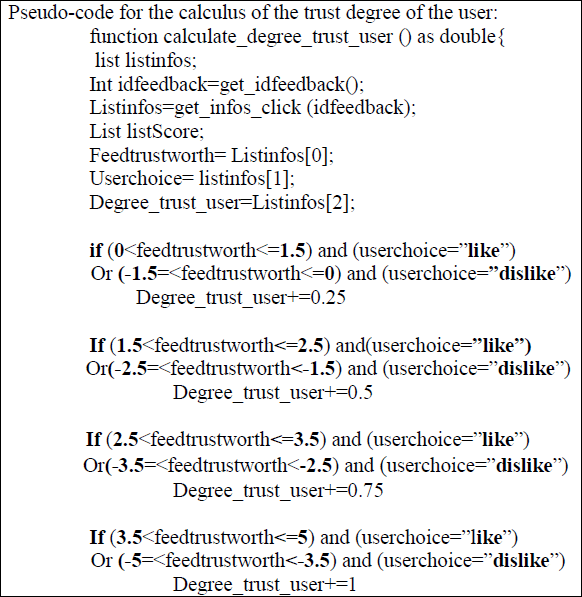
\includegraphics
            [width=0.55\textwidth,keepaspectratio]
            {img/chapter2/trustworthiness_trust_degree_algorithm.png}
            \caption
            [Algorytm określania i~aktualizacji poziomu wiarygodności użytkownika
            przedstawiony w~artykule \cite{article:evaluating_trustworthiness_2013}]
            {Algorytm określania i~aktualizacji poziomu wiarygodności użytkownika
            przedstawiony w~artykule \cite{article:evaluating_trustworthiness_2013}}
            \label{fig:chapter2:przeglad_literatury:artykul_2:trust_degree_algorithm}
        \end{figure}

        Niestety pomimo ciekawego pomysłu, przedstawione rozwiązanie jest mocno
        niedopracowane i~zawiera bardzo ogólną ideę. Wielokrotnie powtarzane jest
        sformułowanie, że w~przyszłych pracach pojawią się dużo bardziej szczegółowe
        i~dopracowane rozwiązania, jednak pomimo upływu czasu od publikacji nic takiego
        nie nastąpiło. Większość realnych problemów jest zasygnalizowane jako sugestia,
        jak np. wykorzystanie pewnych współczynników lub procentów do zmniejszania, lub
        zwiększania poziomu wiarygodności użytkownika. Sama analiza semantyczna, również
        została przedstawiona w~taki sposób, że trzeba ją wykonać, niestety brak jest
        informacji od autorów artykułu o~adaptacji do przedstawionego algorytmu. Nie
        zostały przedstawione również żadne wyniki, które mogłyby świadczyć o~przewadze
        przedstawionej metody w~porównaniu do innych dostępnych rozwiązań. Jest to
        niezwykle ciekawy pomysł, który można rozwinąć w~wielu kierunkach, lecz nie da
        się dokonać analizy wyników, czy kierunek założony przez odbiorców artykułu, jest
        odpowiedni i~przynosi lepsze efekty.

    }

    \section{Metoda kompleksowej analizy reputacji ofert na podstawie aspektowej analizy sentymentu}
    \label{chapter2:przeglad_literatury:artykul_3} {
        Artykuł zatytułowany ''Cross-Platform Reputation Generation System Based on
        Aspect-Based Sentiment Analysis''\cite{article:reputation_generation_system_2022}
        skupia się na przedstawieniu komplementarnego systemu oceny wiarygodności,
        w~którym zostały omówione dokładnie wszystkie aspekty. Warto zaznaczyć, że
        artykuł ten jest niezwykle aktualny, gdyż został opublikowany na początku
        pierwszego kwartału 2022 roku, natomiast autor niniejszej pracy magisterskiej
        przygotowuje ją w~końcówce pierwszego kwartału oraz w~drugim kwartale 2022 roku.

        Autorzy artykułu w~pierwszych sekcjach przedstawiają aktualny stan wiedzy w~tej
        dziedzinie oraz fakt, że naprawdę dostępnych jest wiele prac naukowych
        poruszających ten temat i~proponujących bardzo zróżnicowane metody. Tak jak już
        zostało wspomniane w~ramach analizy pozostałych artykułów w~sekcjach
        \ref{chapter2:przeglad_literatury:artykul_1} oraz
        \ref{chapter2:przeglad_literatury:artykul_2}, wiekszość z~nich opiera się na
        analizie opartej o~wartości numeryczne, w~nowszych pracach są opierane
        o~analizę semantyczną. Niestety ze względu na ograniczenia wynikających z~samej
        koncepcji ocen i~recenzji, nie da się pozyskać więcej informacji.

        Zdaniem autorów proponowane wcześniej metody, czy też algorytmy, bardzo mocno
        skupiały się na samym rdzeniu działania, natomiast były one przedstawione jako
        teoretyczne idee bez konfrontacji z~realną ich implementacją i~wykorzystaniem.
        Co więcej, pomijały one niezwykle kluczowe aspekty takie jak pobieranie
        i~ekstrakcja cech z~konkretnego portalu, czy też wizualizacja uzyskanych wyników,
        aby użytkownik programu implementującego metody mógł w~łatwy i~świadomy sposób
        podjąć decyzję.

        Zdecydowanie warto nadmienić, że artykuł ten porusza dużo szerszy obszar niż
        tylko portale ogłoszeniowe. Źródłem opinii mogą być oczywiście wspomniane
        portale ogłoszeniowe, natomiast niezwykle cenne są również opinii z~takich
        miejsc jak platforma Facebook\cite{website:facebook},
        Instagram\cite{website:instagram}, Twitter\cite{website:twitter},
        YouTube\cite{website:youtube} czy np. TripAdvisor\cite{website:tripadvisor}.
        Niestety w~przypadku wspomnianych serwisów, jest możliwość wystawienia dowolnej
        liczby opinii, nawet w~przypadku niebrania udziału w~wydarzeniu czy też
        korzystania z~danego serwisu czy też portalu. Jest to niezwykle niebezpieczne
        z~punktu widzenia wiarygodności tych opinii i~dalszego sugerowania się nimi
        przy podejmowaniu decyzji.

        Ze względu na powyżej wspomniane kwestie autorzy zaproponowali następujący
        zestaw kroków wykonywanych przez system. Został on zaprezentowany na rysunku
        \ref{fig:chapter2:przeglad_literatury:artykul_3:aspect_based}. Przechodząc do
        omówienia kroku określonego jako filtrowanie pozyskanych opinii, czy też
        recenzji (ang. Spam Filtering) warto podkreślić, że zostały zaproponowane dwa
        sposoby wykrywania. Pierwszym z~nich jest wyliczanie podobieństwa między
        opiniami danej osoby. Zgodnie z~przedstawionymi badaniami, większość osób
        wystawiająca fałszywe opinie dla korzyści finansowych, piszę je w~bardzo
        podobny sposób, często korzystając z~pewnego rodzaju szablonu, aby zwiększyć
        swoją wydajność, a~co za tym idzie zwiększyć swój zysk. Drugim z~nich jest
        wyliczanie wartości wystąpień recenzji danego użytkownika (ang. User Number of
        Reviews Frequency (UNRF)). Podstawą działania jest fakt, że nienaturalnym
        zachowaniem jest wystawianie zbyt dużej liczby recenzji przez jednego
        użytkownika dla wybranego obiektu, oferty czy też usługi. Na podstawie
        przedstawionych w~artykule wzorów są wyliczane wartości (ang. score) dla obu
        sposób i~na tej podstawie jest podejmowana decyzji, czy dany użytkownik jest
        osobą udostępniającą fałszywe recenzje i~oceny, czy też nie. W~przypadku
        uznania, że osoba udostępnia fałszywe informacje zwrotne są one usuwane
        w~procesie filtracji.

        Po przeprowadzeniu kroków wstępnych, opisanych powyżej, wykonywane jest proces
        analizy sentymentu opartej o~aspekty. Polega on na określeniu znaczenia tekstu,
        a~dokładnie to, czy jest pozytywny, czy też negatywny ze względu na przedstawione
        w~tym tekście podmioty. Mogą one być określane przez przymiotniki o~pozytywnych
        i~negatywnych znaczeniach. Ważne jest to, aby brać te podmioty oraz ich
        określenia, które faktycznie są związane z~tym danym obiektem. Przykładem to
        obrazującym jest jakość robionych zdjęć przez aparat oraz jego wygląd. Jakości
        zdjęć często nie można określić przed zakupem, natomiast wygląd jak najbardziej,
        więc nie powinno być to brane pod uwagę przy wyliczaniu znaczenia danej
        wypowiedzi. Sami autorzy przedstawili to w~bardzo ciekawy i~dojmujący sposób,
        tłumacząc zaawansowane kwestie z~tym związane.

        \begin{figure}[H]
            \centering
            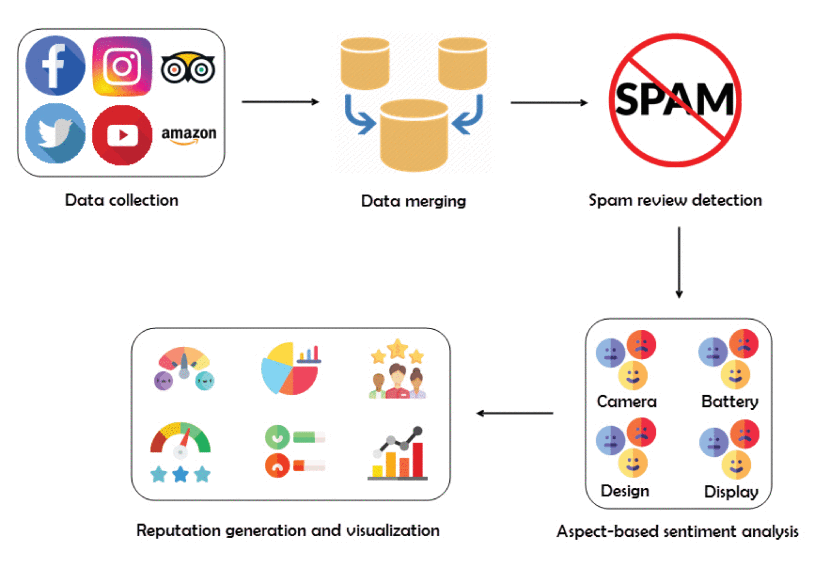
\includegraphics
            [width=0.55\textwidth,keepaspectratio]
            {img/chapter2/aspect_based_sentiment_analysis.png}
            \caption
            [Zestaw kroków przeprowadzanych przez proponowany system reputacji
            przedstawiony w~artykule \cite{article:reputation_generation_system_2022}]
            {Zestaw kroków przeprowadzanych przez proponowany system reputacji
            przedstawiony w~artykule \cite{article:reputation_generation_system_2022}}
            \label{fig:chapter2:przeglad_literatury:artykul_3:aspect_based}
        \end{figure}

        Przedstawione powyżej biegunowość jest jedną z~wartości branych pod uwagę przy
        wyliczaniu reputacji, oprócz niej są jeszcze dwie. Pierwszą z~nich, jest
        wartość popularności danej opinii, czy też recenzji, wyliczana na podstawie
        liczby polubień i~udostępnień. Podstawą do brania tego pod uwagę jest fakt, że
        jeżeli ktoś polubił daną opinię to najprawdopodobniej się z~nią zgadza lub
        uznał ją za przydatną w~procesie podejmowania decyzji. Drugą wartością jest
        data wystawienia danej informacji zwrotnej, im jest starsza tym jest większe
        prawdopodobieństwo tego, że jest nieaktualna lub jej zawartość może nie do
        końca zgadzać się z~teraźniejszym stanem. Powodem tego może być to, że np.
        sprzedawca poprawił lub pogorszył jakość usług, lub produktu. Możliwe jest też
        to, że zmienił np. opis, dzięki czemu teraz każdy klient jest dokładnie
        poinformowany o~newralgicznych kwestiach.

        Na podstawie tych trzech wartości jest obliczany wartość reputacji (ang.
        reputation score) i~jest ona przedstawiona użytkownikowi w~graficznej formie
        razem z~podziałem wartości analizy sentymentu na aspekty. Co więcej,
        najbardziej wiarygodne opinie lub recenzje są wyświetlane, celem potwierdzenia
        przedstawionych wartości liczbowych.

        W~artykule w~bardzo przystępny sposób zostały przedstawione eksperymenty,
        wartości parametrów i~hiperparametrów oraz uzyskane wyniki. Same zbiory danych
        wykorzystane do badań zawierają zagregowane opinie o~np. hotelu
        z~przedstawionych powyżej portali TripAdvisor, Facebook czy Twitter lub
        dotyczące filmu, pobrane z~portalu IMDb oraz z~Facebook i~Twitter.

    }

    \section{Potencjalne obszary ulepszeń obecnie dostępnych rozwiązań}
    \label{chapter2:przeglad_literatury:ulepszenia} {
        Artykuły przedstawione w~sekcjach \ref{chapter2:przeglad_literatury:artykul_1},
        \ref{chapter2:przeglad_literatury:artykul_2} oraz
        \ref{chapter2:przeglad_literatury:artykul_3} zawierają bardzo ciekawe pomysły,
        często ich implementacje oraz wyniki. Bazują one na innych, wcześniej
        przedstawionych pracach i~je rozwijają lub pokazują zupełnie inne podejście,
        mając na uwadzę dotychczasowy stan wiedzy w~tej dziedzinie.

        Autor niniejszej pracy dyplomowej po dogłębnych poszukiwaniach w~dostępnych
        bazach literatury naukowej, przeczytaniu dziesiątek artykułów, które zostały
        wybrane po wstępnej selekcji na podstawie istotności w~stosunku do tematu tej
        pracy, postanowił przedstawić potencjalne obszary ulepszeń.

        Zdaniem autora niniejszej pracy dyplomowej można wykorzystać wszystkie dostępne
        informacje, jakie zapewnia dany portal ogłoszeniowy. Są to informacje
        w~formie wartości liczbowych takich jak cena, średnia ocena klientów, oceny
        o~sprzedawcy w~różnych kategoriach takich jak szybkość dostawy, dokładność
        opisu. Co więcej, można przeprowadzić analizę semantyczną zawartości tekstowej,
        nie ograniczając się do zwykłej biegunowości, czyli czy ocena jest
        pozytywna lub negatywna. Istnieje możliwość badania emocji na podstawie słów
        użytych przez autora recenzji. Zebrane tak dane, można poddać procesowi
        grupowania poprzez skorzystanie z~jednego z~wybranych algorytmów zapewniających
        taką możliwość. Wynikiem grupowanie byłyby dwa klastry z~ofertami o~wysokiej lub
        niskiej reputacji. Podejście to rozwiązuje problem dobierania współczynników,
        które dla różnych zbiorów mogą być zdecydowanie inne, aby uzyskiwać zadowalające
        efekty.

    }

}
\end{document}
